\let\negmedspace\undefined
\let\negthickspace\undefined
\documentclass[journal]{IEEEtran}
\usepackage[a5paper, margin =  10mm, onecolumn]{geometry}
%\usepackage{lmodern} % Ensure lmodern is loaded for pdflatex
\usepackage{tfrupee} % Include tfrupee package

\setlength{\headheight}{1cm} % Set the height of the header box
\setlength{\headsep}{0mm}     % Set the distance between the header box and the top of the text

\usepackage{gvv-book}
\usepackage{gvv}
\usepackage{cite}
\usepackage{amsmath,amssymb,amsfonts,amsthm}
\usepackage{algorithmic}
\usepackage{graphicx}
\usepackage{textcomp}
\usepackage{xcolor}
\usepackage{txfonts}
\usepackage{listings}
\usepackage{enumitem}
\usepackage{mathtools}
\usepackage{gensymb}
\usepackage{comment}
\usepackage[breaklinks =  true]{hyperref}
\usepackage{tkz-euclide} 
\usepackage{listings}
% \usepackage{gvv}                                        
\def\inputGnumericTable{}                                 
\usepackage[latin1]{inputenc}                                
\usepackage{color}                                            
\usepackage{array}                                            
\usepackage{longtable}                                       
\usepackage{calc}                                             
\usepackage{multirow}                                         
\usepackage{hhline}                                           
\usepackage{ifthen}                                           
\usepackage{lscape}
\begin{document}

\bibliographystyle{IEEEtran}
\vspace{3cm}

\title{2.4.31}
\author{EE25BTECH11034 - Kishora Karthik}
% \maketitle
% \newpage
% \bigskip
{\let\newpage\relax\maketitle}

\renewcommand{\thefigure}{\theenumi}
\renewcommand{\thetable}{\theenumi}
%\setlength{\intextsep}{10pt} % Space between text and floats
\textbf{Question:}\\
Check if the point $\vec{A}(2, 7)$ lies on the perpendicular bisector of line segment joining the points
$\vec{P}(6, 5)$ and $\vec{Q}(0, -4)$.\\\\
\textbf{Formulae}:\\
The equation of the perpendicular bisector of PQ is\\
\begin{align}
    \brak{\vec{A}-\frac{\vec{P}+\vec{Q}}{2}}^\top\brak{\vec{P}-\vec{Q}}=0
\end{align}
\textbf{Solution:}
The given points are,\\
\begin{align}
    \vec{A}=\myvec{2\\7}\\
    \vec{P}=\myvec{6\\5}\\
    \vec{Q}=\myvec{0\\-4}
\end{align}
\begin{align}
    \vec{P}-\vec{Q}=\myvec{6\\5}-\myvec{0\\-4}\\
    \vec{P}-\vec{Q}=\myvec{6\\9}
\end{align}
\begin{align}
    \frac{\vec{P}+\vec{Q}}{2}={\frac{\myvec{6\\5}+\myvec{0\\-4}}{2}}
\end{align}
\begin{align}
    \frac{\vec{P}+\vec{Q}}{2}={\frac{\myvec{6\\1}}{2}}\\
    \frac{\vec{P}+\vec{Q}}{2}=\myvec{3\\0.5}   
\end{align}
\begin{align}
    \vec{A}-\frac{\vec{P}+\vec{Q}}{2}=\myvec{2\\7}-\myvec{3\\0.5} 
\end{align}
\begin{align}
    \vec{A}-\frac{\vec{P}+\vec{Q}}{2}=\myvec{-1\\6.5}   
\end{align}
\begin{align}
    \brak{\vec{A}-\frac{\vec{P}+\vec{Q}}{2}}^\top\brak{\vec{P}-\vec{Q}}=\myvec{-1&6.5}\myvec{6\\9}
\end{align}
\begin{align}
    \brak{\vec{A}-\frac{\vec{P}+\vec{Q}}{2}}^\top\brak{\vec{P}-\vec{Q}}=(-1)(6)+(6.5)(9)
\end{align}
\begin{align}
    \brak{\vec{A}-\frac{\vec{P}+\vec{Q}}{2}}^\top\brak{\vec{P}-\vec{Q}}=52.5\neq0
\end{align}
The equation of perpendicular bisector is not satisfied.\\
Therefore, point $\vec{A}$ does not lie on the perpendicular bisector of line segment joining the points $\vec{P}$ and $\vec {Q}$.\\

\centering
    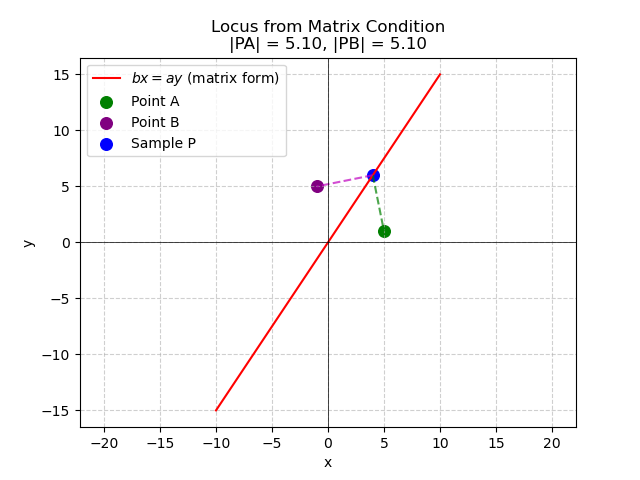
\includegraphics[width=\columnwidth, height=0.8\textheight, keepaspectratio]{Figs/Fig1.png} 

\end{document}

